\subsection{Parametros do dataset}


\quad In the following image we have a print of the columns of the dataset mentioned above:

\begin{figure}[H]
    \centering
    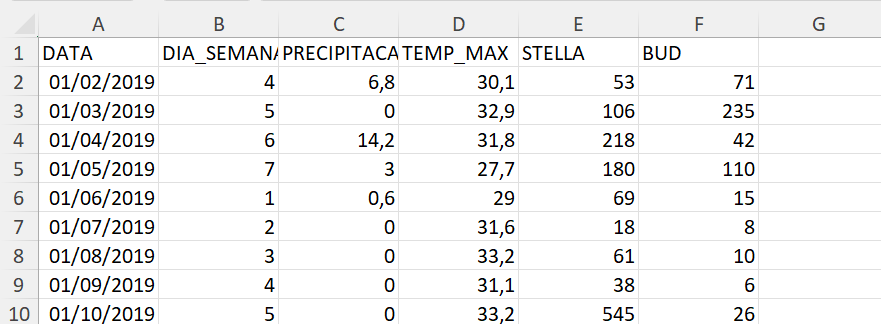
\includegraphics[width=0.8\textwidth]{assets/dataset.png}
    \caption{Project Dataset}
    \label{fig:dataset}
    \end{figure}

\quad The following dataset is compose of 6 columns, they being:

\quad \quad \textbullet DATA: This column represents the date the records are from;

\quad \quad \textbullet DIA\_SEMANA: This column represents the day of the week, where 1 is Sunday, 2 is Monday, 3 is Tuesday, 4 is Wednesday, 5 is Thursday, 6 is Friday and 7 is Saturday;

\quad \quad \textbullet PRECIPITACAO: This column represents the total of precipitation in mm in that day;

\quad \quad \textbullet TEMP\_MAX: This column represents the daily maximum temperature in Celcius from that day;

\quad \quad \textbullet STELLA: This column represents the number of STELLA drinks that where sold in that day;

\quad \quad \textbullet BUD: This column represents the number of BUD drinks that where sold in that day.
